\chapter{Dasar Dasar Code OpenCV}
\section{Menampilkan gambar}
\subsection{Menampilkan Gambar}

\lstinputlisting{src/cv2.py}
\begin{enumerate}
	\item lakukan Import library open cv yaitu cv2
	\item kemudian panggil file foto menggunakan kode seperti di atas, membuat terlebihdahulu variabel img, kemudian cv2.imread nama file dan nomor untuk gradiasi warnanya, pada bagian ini menggunakan angka 1 yang artinya mengikuti foto aslinya.
	\item lakukan print untuk menampilkan gambar
	\item kemudian buat frame untuk menampilkan gambar menggunakan imshow dengan nama frame image.
	\item kemudian gunakan waitKey untuk membuat frame agar tidak langsung mati atau tertutup otomatis.
	\item destroyAllWindows digunakan untuk menutup frame.
\end{enumerate}

\begin{figure}[ht]
\centering
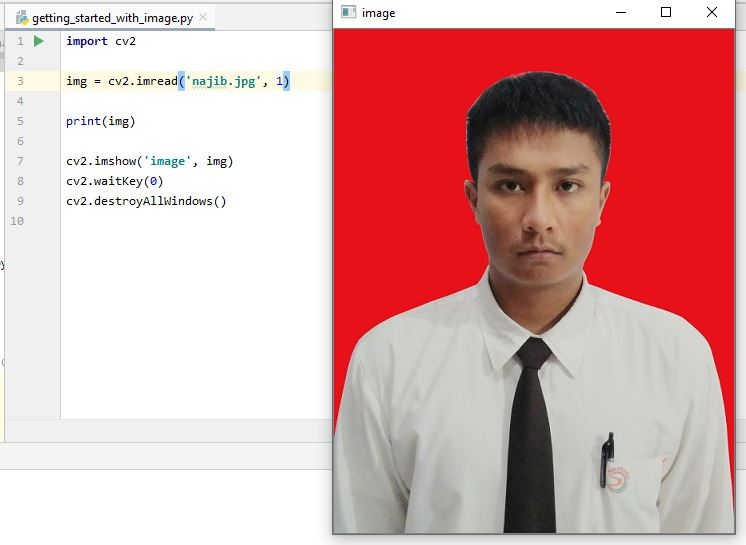
\includegraphics[scale=0.5]{figures/2,2.jpg}
\caption{Menampilkan gambar}
\label{contoh}
\end{figure}
Hasil yang ditampilkan sama seperti foto aslinya karna tidak ada dari foto yang di rubah sama sekali, kodingan ini hanya bertujuan untuk menampilkan gambar saja.

\newpage
\subsection{Menampilkan Gambar dan merubah kontras warnanya}
\lstinputlisting{src/cv1.py}
\begin{enumerate}
	\item lakukan Import library open cv yaitu cv2
	\item kemudian panggil file foto menggunakan kode seperti di atas, membuat terlebihdahulu variabel img, kemudian cv2.imread nama file dan nomor untuk gradiasi warnanya, pada bagian ini menggunakan angka 0 merubah gambar menjadi hitam putih.
	\item lakukan print untuk menampilkan gambar
	\item kemudian buat frame untuk menampilkan gambar menggunakan imshow dengan nama frame image.
	\item kemudian gunakan waitKey untuk membuat frame agar tidak langsung mati atau tertutup otomatis.
	\item destroyAllWindows digunakan untuk menutup frame.
\end{enumerate}


\begin{figure}[ht]
\centering
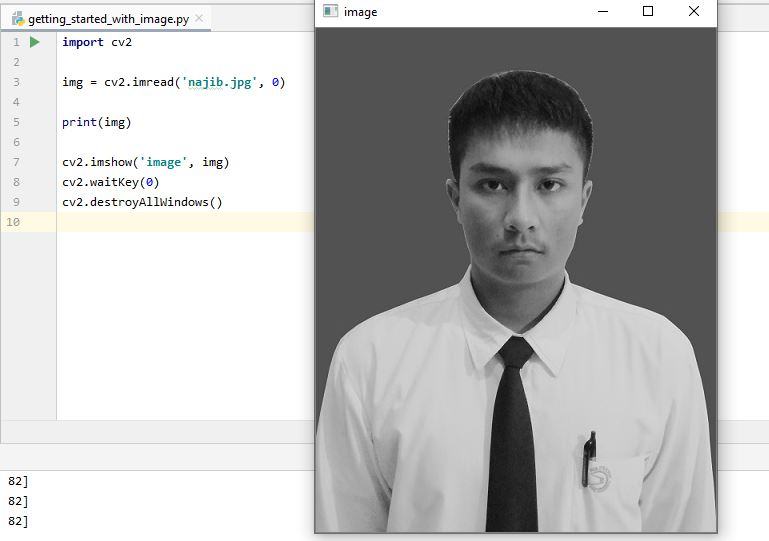
\includegraphics[scale=0.5]{figures/2,1.jpg}
\caption{Merubah kontras warna}
\label{contoh}
\end{figure}

Pada bagian kodingan ini foto di rubah kontras warnanya menjadi hitam putih, pada kodingan sebelumnya yang di rubah hanya satu huruf saja untu menjadikan foto ini menjadi seperti ini. yaitu pada bagian imread nya menjadi 0.

\subsection{Menyimpan Gambar menggunakan kode opencv}
\lstinputlisting{src/cv3.py}
\begin{enumerate}
	\item lakukan Import library open cv yaitu cv2
	\item kemudian panggil file foto menggunakan kode seperti di atas, membuat terlebihdahulu variabel img, kemudian cv2.imread nama file dan nomor untuk gradiasi warnanya, pada bagian ini menggunakan angka 0 merubah gambar menjadi hitam putih.
	\item lakukan print untuk menampilkan gambar
	\item kemudian buat frame untuk menampilkan gambar menggunakan imshow dengan nama frame image.
	\item kemudian gunakan waitKey untuk membuat frame agar tidak langsung mati atau tertutup otomatis.
	\item destroyAllWindows digunakan untuk menutup frame.
	\item terakhir gambar disimpan menggunakan kode imwrite, pertama tuliskan nama gambar yang akan disimpan beserta formatgambarnya, kemudian kode img untuk menyatakan yang disimpan tersebut adalah gambar.
\end{enumerate}

\newpage
\begin{figure}[ht]
\centering
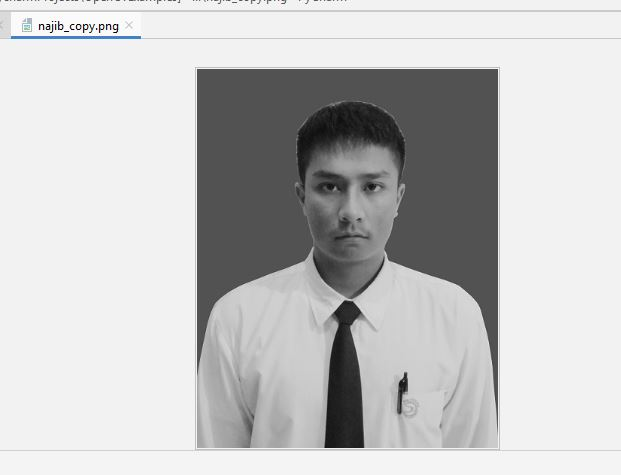
\includegraphics[scale=0.5]{figures/2,3.jpg}
\caption{Menyimpan gambar}
\label{contoh}
\end{figure}

Gambar berhasil disimpan dengan nama najibcopy.png, gambar disimpan sesuai yang telah di edit kontras warnanya menjadi hitam putih sesuai cede yang kita jalankan.

\newpage
\section{Menjalankan kamera leptop}
\subsection{Menjalankan video kamera leptop}
\lstinputlisting{src/cv4.py}
\begin{enumerate}
	\item lakukan Import library open cv yaitu cv2
	\item kemudian buat variable baru dengan nama cap kemudian panggil VideoCapture(0) yang artinya menjalankan kamera leptop.
	\item membuat while yaitu perulangan membuka frame
	\item kemudian didalam perulangan tersebut terdapat frame yang membaca atau merekam video.
	\item kemudian buat frame dengan nama frame
	\item kemudian gunakan waitKey untuk membuat frame agar tidak langsung mati atau tertutup otomatis.
	\item release untuk menutup videocapture
	\item destroyAllWindows digunakan untuk menutup frame.
\end{enumerate}

\newpage
\begin{figure}[ht]
\centering
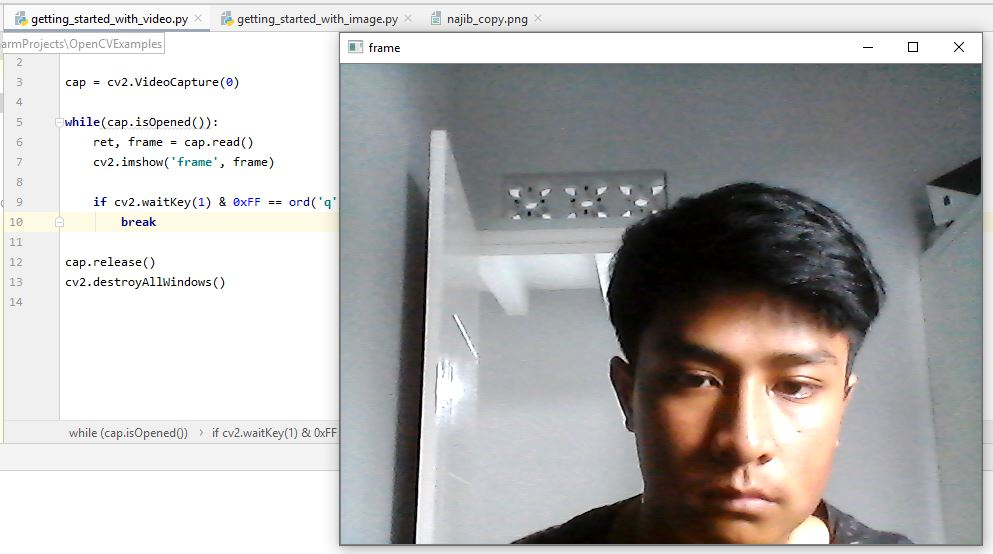
\includegraphics[scale=0.5]{figures/2,4.jpg}
\caption{Menggunakan kamera leptop}
\label{contoh}
\end{figure}

Pada videocpture ini hanya merekam menggunakan kamera leptop saja belum masuk ke pengolahan gambar.

\newpage
\subsection{Merubah kontras warna pada video}
\lstinputlisting{src/cv5.py}
\begin{enumerate}
	\item lakukan Import library open cv yaitu cv2
	\item kemudian buat variable baru dengan nama cap kemudian panggil VideoCapture(0) yang artinya menjalankan kamera leptop.
	\item membuat while yaitu perulangan membuka frame
	\item kemudian didalam perulangan tersebut terdapat frame yang membaca atau merekam video.
	\item buat variable dengan nama gray karna kita mau berubah kontras warnanya menjadi hitam putih, kemudian panggil cvtColor didalam frame dengan warna abu abu.
	\item kemudian buat frame dengan nama frame
	\item kemudian gunakan waitKey untuk membuat frame agar tidak langsung mati atau tertutup otomatis.
	\item release untuk menutup videocapture
	\item destroyAllWindows digunakan untuk menutup frame.
\end{enumerate}

\begin{figure}[ht]
\centering
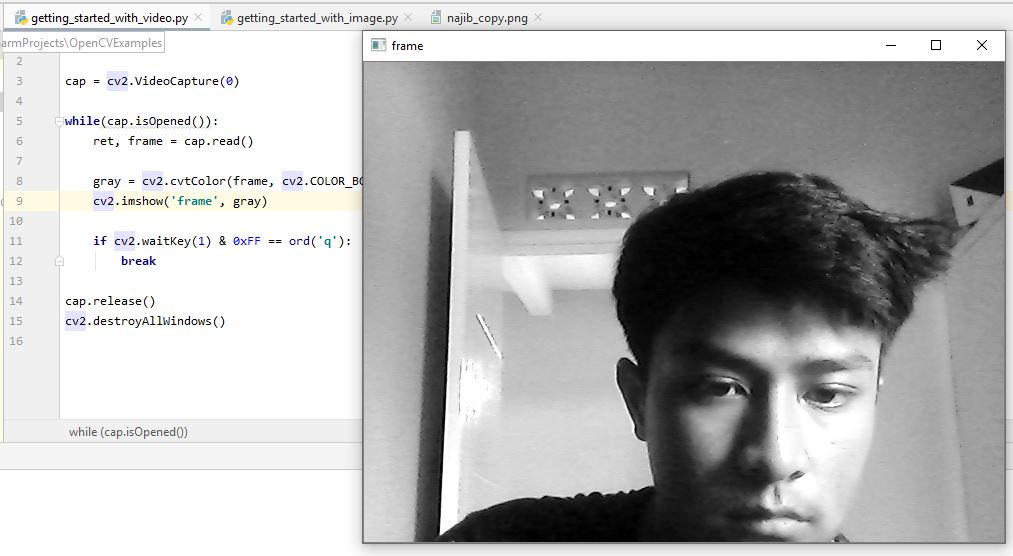
\includegraphics[scale=0.5]{figures/2,5.jpg}
\caption{Kontras warna video}
\label{contoh}
\end{figure}

Pada videocpture ini video sudah di rubah kontras warnanya menjadi abu abu, kita bisa rubah sesuai yang kita inginkan.

\newpage
\subsection{Mengetahui ukuran frame yang ditampilkan}
\lstinputlisting{src/cv6.py}
\begin{enumerate}
	\item lakukan Import library open cv yaitu cv2
	\item kemudian buat variable baru dengan nama cap kemudian panggil VideoCapture(0) yang artinya menjalankan kamera leptop.
	\item membuat while yaitu perulangan membuka frame
	\item kemudian didalam perulangan tersebut terdapat frame yang membaca atau merekam video.
	\item kita cukup print mengambil dari videocapture dan panggil CAP PROP FRAME WIDTH untuk mengetahui ukuran lebarnya dan CAP PROP FRAME HEIGHT untuk ukuran tingginya 
	\item buat variable dengan nama gray karna kita mau berubah kontras warnanya menjadi hitam putih, kemudian panggil cvtColor didalam frame dengan warna abu abu.
	\item kemudian buat frame dengan nama frame
	\item kemudian gunakan waitKey untuk membuat frame agar tidak langsung mati atau tertutup otomatis.
	\item release untuk menutup videocapture
	\item destroyAllWindows digunakan untuk menutup frame.
\end{enumerate}

\newpage
\begin{figure}[ht]
\centering
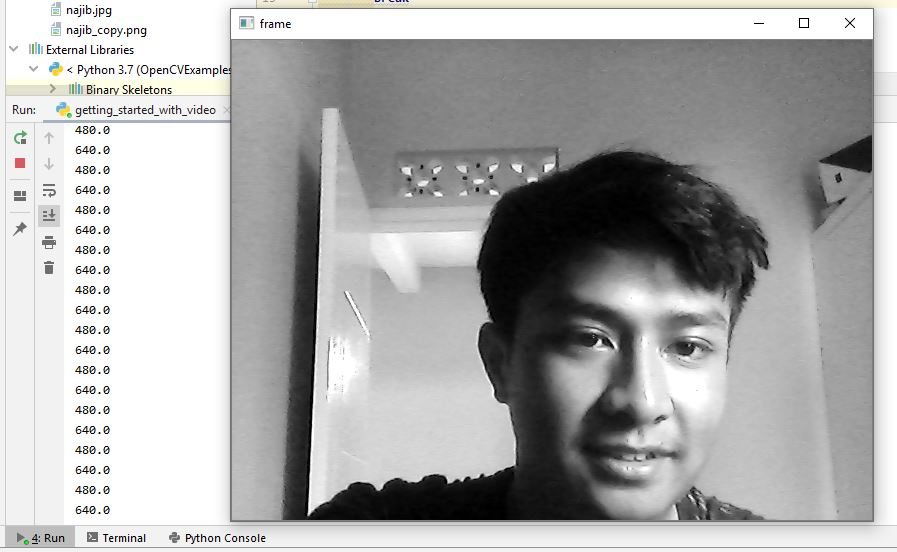
\includegraphics[scale=0.5]{figures/2,6.jpg}
\caption{Ukuran Frame video}
\label{contoh}
\end{figure}

Maka akan ditampilkan secara berulang karna berada pada while dan pada bagian videocapture juga jika tidak di lakukan perulangan maka sekali muncul akan langsung keluar secara otomatis.

\newpage
\subsection{Menyimpan video}
\lstinputlisting{src/cv7.py}
\begin{enumerate}
	\item lakukan Import library open cv yaitu cv2
	\item kemudian buat variable baru dengan nama cap kemudian panggil VideoCapture(0) yang artinya menjalankan kamera leptop.
	\item membuat variabel fourcc untuk merekam video yang dijalankan.
	\item membuat variable out untuk menyimpan video dengan nama najib.avi dan frame berukuran 640,480.
	\item melakukan print apakah true atau false kamera leptop terbuka.
	\item membuat while yaitu perulangan membuka frame
	\item kemudian didalam perulangan tersebut terdapat frame yang membaca atau merekam video.
	\item jika kamera true merekam maka akan melakukan perintah.
	\item kita cukup print mengambil dari videocapture dan panggil CAP PROP FRAME WIDTH untuk mengetahui ukuran lebarnya dan 
	\item kita cukup print mengambil dari videocapture dan panggil CAP PROP FRAME HEIGHT untuk ukuran tingginya 
	\item buat variable dengan nama gray karna kita mau berubah kontras warnanya menjadi hitam putih, kemudian panggil cvtColor didalam frame dengan warna abu abu.
	\item kemudian buat frame dengan nama frame
	\item kemudian gunakan waitKey untuk membuat frame agar tidak langsung mati atau tertutup otomatis.
	\item release untuk menutup videocapture
	\item destroyAllWindows digunakan untuk menutup frame.
\end{enumerate}

\begin{figure}[ht]
\centering
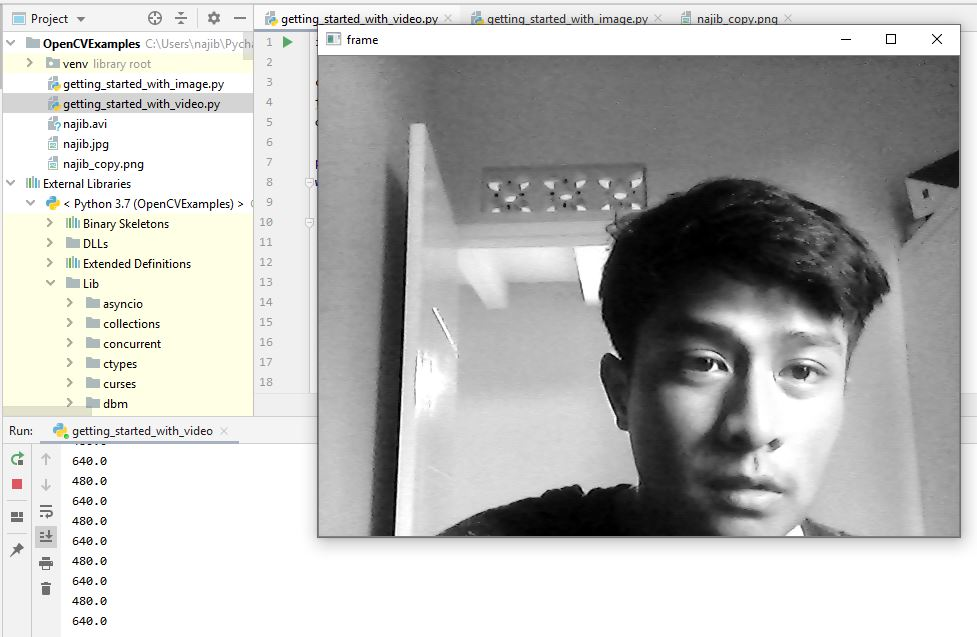
\includegraphics[scale=0.5]{figures/2,7.jpg}
\caption{Setelah dijalankan file tersimpan}
\label{contoh}
\end{figure}

\newpage
\begin{figure}[ht]
\centering
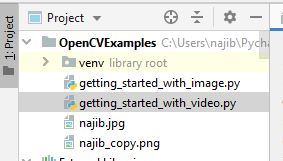
\includegraphics[scale=0.5]{figures/2,7,1.jpg}
\caption{File Sebelum dijalankan}
\label{contoh}
\end{figure}

\begin{figure}[ht]
\centering
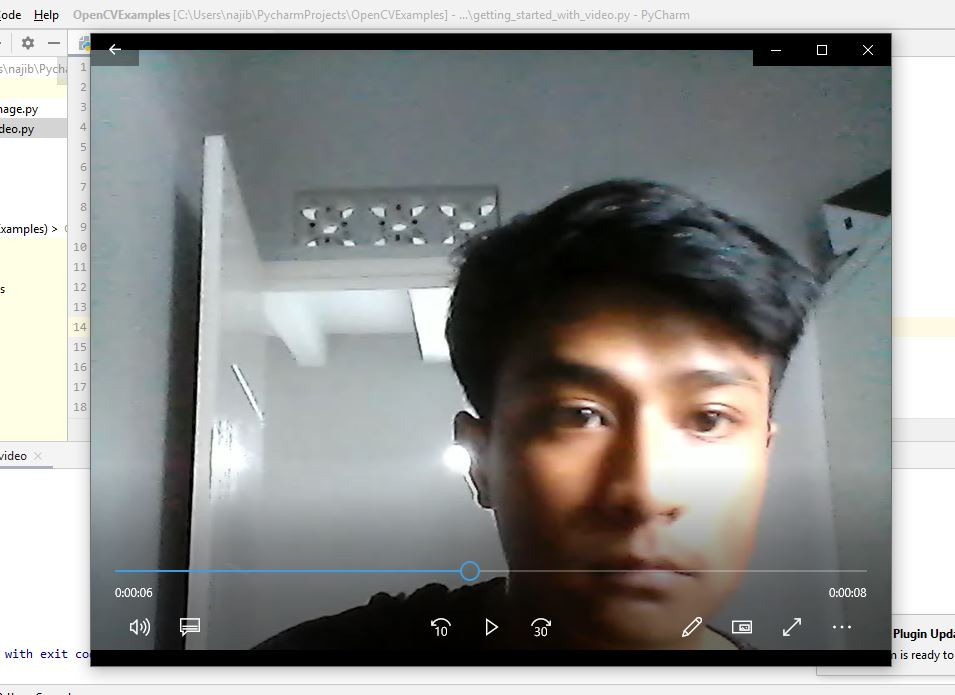
\includegraphics[scale=0.5]{figures/2,7,2.jpg}
\caption{Video yang sudah di simpan}
\label{contoh}
\end{figure}

Video tersimpan langsung ke folder yang dituju, video dapat disesuaikan formatnya sesuai yang kita mau.

\newpage
\section{Menggambar Geometric Pada Foto}
\subsection{Membuat garis}
\lstinputlisting{src/cv8.py}
\begin{enumerate}
	\item lakukan Import library open cv yaitu cv2
	\item kemudian panggil file foto menggunakan kode seperti di atas, membuat terlebihdahulu variabel img, kemudian cv2.imread nama file dan nomor untuk gradiasi warnanya, pada bagian ini menggunakan angka 0 yang artinya gambar berubah menjadi hitam putih.
	\item kemudian buat garis menggunakan cv2.line, 0,0 merupakan dimana titik awal garis tersebut dan 255,255 merupakan titik akhir dari garis tersebut, kemudian selanjutnya adahal warna dari garis tersebut, dan yang terakhir adalah ketebalan dari garis yang dibuat.
	\item kemudian buat frame untuk menampilkan gambar menggunakan imshow dengan nama frame image.
	\item kemudian gunakan waitKey untuk membuat frame agar tidak langsung mati atau tertutup otomatis.
	\item destroyAllWindows digunakan untuk menutup frame.
\end{enumerate}

\newpage
\begin{figure}[ht]
\centering
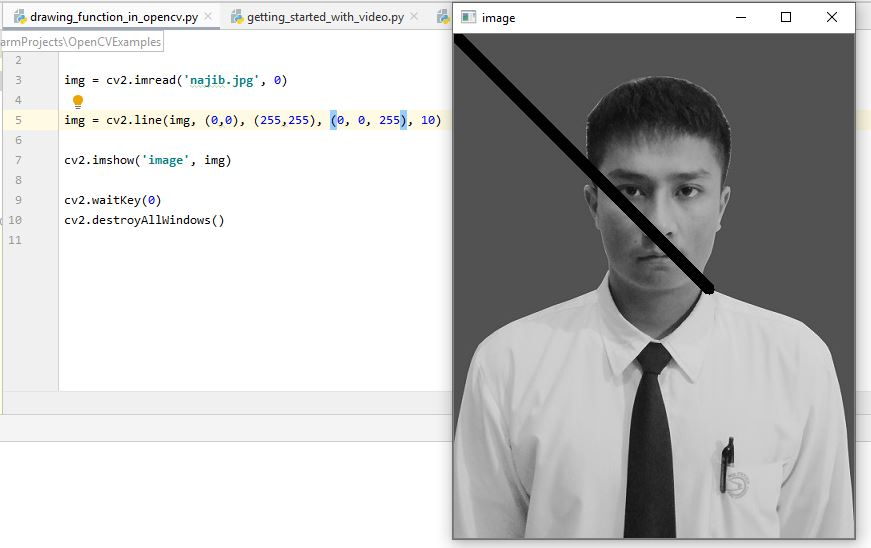
\includegraphics[scale=0.5]{figures/2,8.jpg}
\caption{MMembuat garis}
\label{contoh}
\end{figure}

garis bisa kita taruh dimana saja sesuai yang diinginkan kenapa garisnya menjulur dari pojok kiri atas ke tengah karna titik 0,0 berada di pojok kiri atas sedangkan titik 255,255 berada di tengah tengah gambar, gambar ini pun menjadi hitam putih karna di awal pada imread nya diberikan angka 0 yang membuat gambar berubah menjadi hitam putih.

\newpage
\subsection{Membuat warna warna pada garis}
\lstinputlisting{src/cv9.py}
\begin{enumerate}
	\item lakukan Import library open cv yaitu cv2
	\item kemudian panggil file foto menggunakan kode seperti di atas, membuat terlebihdahulu variabel img, kemudian cv2.imread nama file dan nomor untuk gradiasi warnanya, pada bagian ini menggunakan angka 1 yang artinya mengikuti foto aslinya.
	\item kemudian buat garis menggunakan cv2.line, 0,0 merupakan dimana titik awal garis tersebut dan 255,255 merupakan titik akhir dari garis tersebut, kemudian selanjutnya adalah warna dari garis tersebut, dan yang terakhir adalah ketebalan dari garis yang dibuat.
	\item kemudian buat frame untuk menampilkan gambar menggunakan imshow dengan nama frame image.
	\item kemudian gunakan waitKey untuk membuat frame agar tidak langsung mati atau tertutup otomatis.
	\item destroyAllWindows digunakan untuk menutup frame.
\end{enumerate}

\newpage
\begin{figure}[ht]
\centering
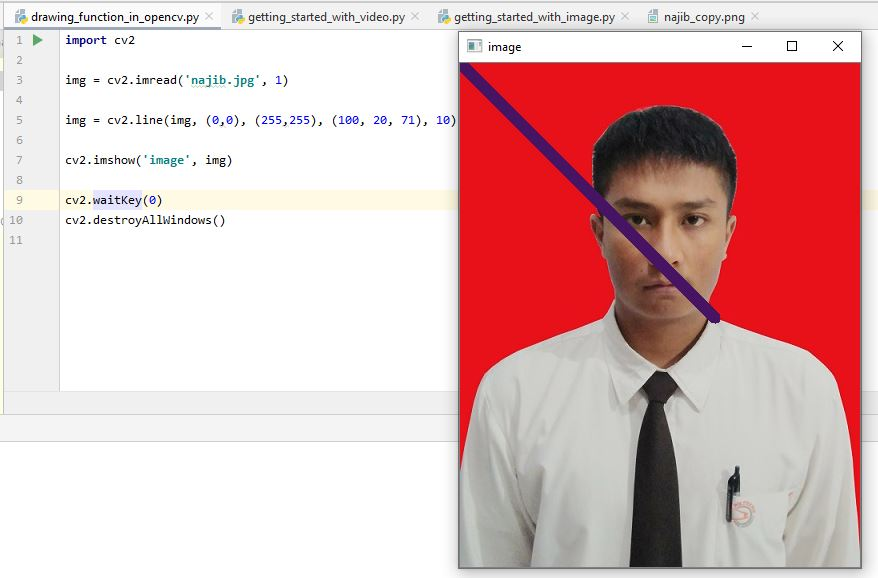
\includegraphics[scale=0.5]{figures/2,9.jpg}
\caption{Membuat garis}
\label{contoh}
\end{figure}

garis bisa kita taruh dimana saja sesuai yang diinginkan kenapa garisnya menjulur dari pojok kiri atas ke tengah karna titik 0,0 berada di pojok kiri atas sedangkan titik 255,255 berada di tengah tengah gambar, gambar menjadi seperti aslinya karna pada imreadnya 1.

\newpage
\begin{figure}[ht]
\centering
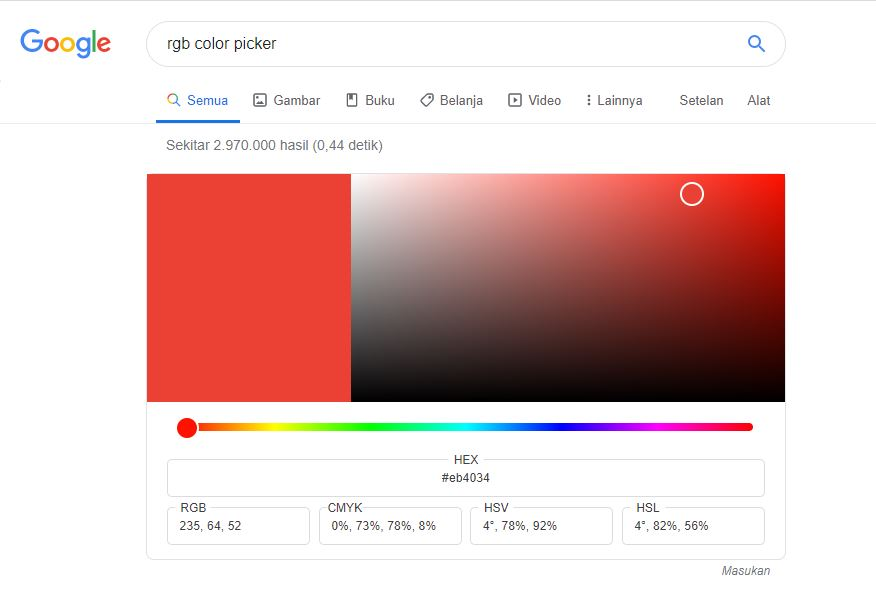
\includegraphics[scale=0.5]{figures/2,9,1.jpg}
\caption{Nomor Nomor warna}
\label{contoh}
\end{figure}

jika kita ingin warna yang sesuai dengan keinginan kita, kita bisa langsung search di google seperti pada gambar maka akan ada nomor nomornya untuk setiap warna.

\newpage
\subsection{Membuat garis panah}
\lstinputlisting{src/cv10.py}
\begin{enumerate}
	\item lakukan Import library open cv yaitu cv2
	\item kemudian panggil file foto menggunakan kode seperti di atas, membuat terlebihdahulu variabel img, kemudian cv2.imread nama file dan nomor untuk gradiasi warnanya, pada bagian ini menggunakan angka 1 yang artinya mengikuti foto aslinya.
	\item kemudian buat garis menggunakan cv2.line, 0,0 merupakan dimana titik awal garis tersebut dan 255,255 merupakan titik akhir dari garis tersebut, kemudian selanjutnya adalah warna dari garis tersebut, dan yang terakhir adalah ketebalan dari garis yang dibuat.
	\item kemudian buat garis panah menggunakan cv2.arrowedLine, 0,0 merupakan dimana titik awal garis tersebut dan 255,255 merupakan titik akhir dari garis tersebut, kemudian selanjutnya adalah warna dari garis tersebut, dan yang terakhir adalah ketebalan dari garis yang dibuat.
	\item kemudian buat frame untuk menampilkan gambar menggunakan imshow dengan nama frame image.
	\item kemudian gunakan waitKey untuk membuat frame agar tidak langsung mati atau tertutup otomatis.
	\item destroyAllWindows digunakan untuk menutup frame.
\end{enumerate}

\newpage
\begin{figure}[ht]
\centering
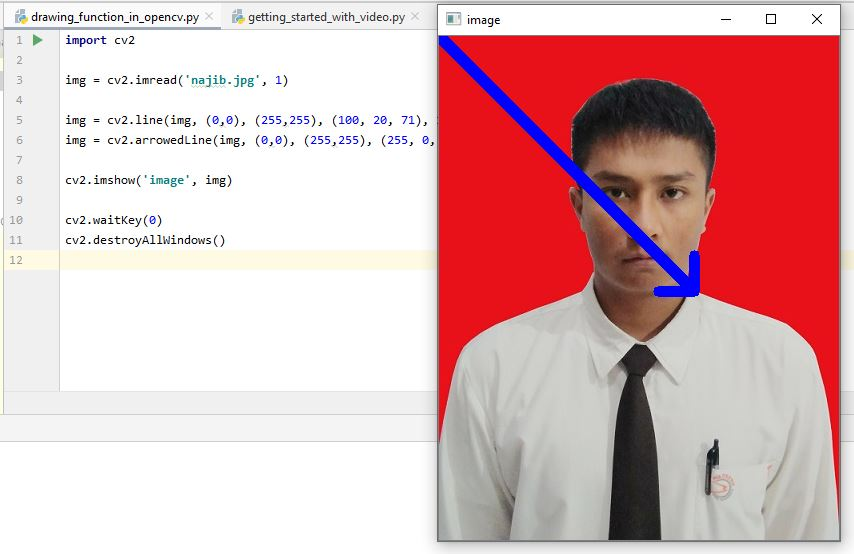
\includegraphics[scale=0.5]{figures/2,10.jpg}
\caption{Membuat garis panah}
\label{contoh}
\end{figure}

Garis panah yang dibuat menumpuk dengan garis yang awal jadi yang di lihat seperti garis yang sebelumnya hilang padahal garis tersebut tertumpuk.

\newpage
\subsection{Membuat garis kotak}
\lstinputlisting{src/cv11.py}
\begin{enumerate}
	\item lakukan Import library open cv yaitu cv2
	\item kemudian panggil file foto menggunakan kode seperti di atas, membuat terlebihdahulu variabel img, kemudian cv2.imread nama file dan nomor untuk gradiasi warnanya, pada bagian ini menggunakan angka 1 yang artinya mengikuti foto aslinya.
	\item kemudian buat garis menggunakan cv2.line, 0,0 merupakan dimana titik awal garis tersebut dan 255,255 merupakan titik akhir dari garis tersebut, kemudian selanjutnya adalah warna dari garis tersebut, dan yang terakhir adalah ketebalan dari garis yang dibuat.
	\item kemudian buat garis panah menggunakan cv2.arrowedLine, 0,0 merupakan dimana titik awal garis tersebut dan 255,255 merupakan titik akhir dari garis tersebut, kemudian selanjutnya adalah warna dari garis tersebut, dan yang terakhir adalah ketebalan dari garis yang dibuat.
	\item kemudian buat garis kotak menggunakan cv2.rectangle, 384,0 merupakan dimana titik awal garis tersebut dan 210,210 merupakan titik akhir dari garis tersebut, kemudian selanjutnya adalah warna dari garis tersebut, dan yang terakhir adalah ketebalan dari garis yang dibuat.
	\item kemudian buat frame untuk menampilkan gambar menggunakan imshow dengan nama frame image.
	\item kemudian gunakan waitKey untuk membuat frame agar tidak langsung mati atau tertutup otomatis.
	\item destroyAllWindows digunakan untuk menutup frame.
\end{enumerate}

\newpage
\begin{figure}[ht]
\centering
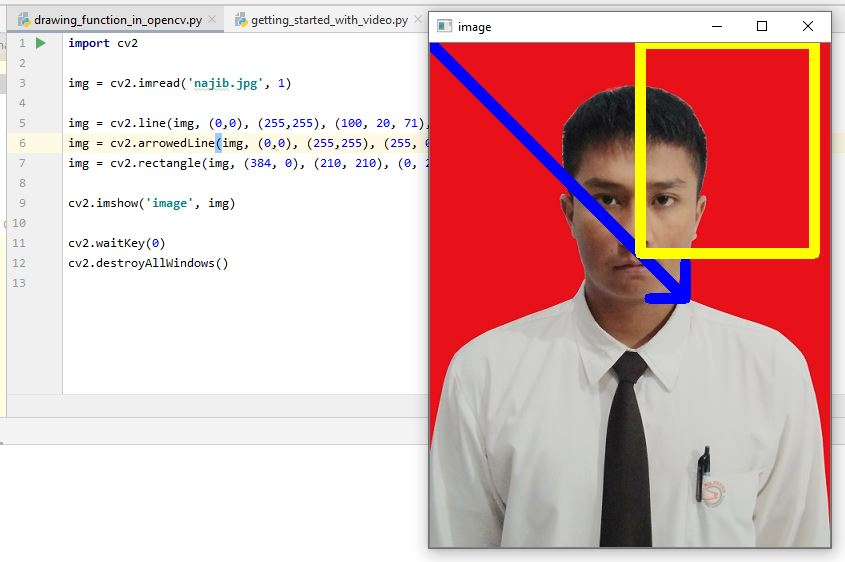
\includegraphics[scale=0.5]{figures/2,11.jpg}
\caption{Membuat garis kotak}
\label{contoh}
\end{figure}

Garis kotak ini bisa kita atur mau warna yang bagaimana, ukuran yang bagaimana, dan posisi yang bagaimana sesuai yang di inginkan dan sesuai kebutuhannya.

\newpage
\subsection{Membuat kotak}
\lstinputlisting{src/cv12.py}
\begin{enumerate}
	\item lakukan Import library open cv yaitu cv2
	\item kemudian panggil file foto menggunakan kode seperti di atas, membuat terlebihdahulu variabel img, kemudian cv2.imread nama file dan nomor untuk gradiasi warnanya, pada bagian ini menggunakan angka 1 yang artinya mengikuti foto aslinya.
	\item kemudian buat garis menggunakan cv2.line, 0,0 merupakan dimana titik awal garis tersebut dan 255,255 merupakan titik akhir dari garis tersebut, kemudian selanjutnya adalah warna dari garis tersebut, dan yang terakhir adalah ketebalan dari garis yang dibuat.
	\item kemudian buat garis panah menggunakan cv2.arrowedLine, 0,0 merupakan dimana titik awal garis tersebut dan 255,255 merupakan titik akhir dari garis tersebut, kemudian selanjutnya adalah warna dari garis tersebut, dan yang terakhir adalah ketebalan dari garis yang dibuat.
	\item kemudian buat garis kotak menggunakan cv2.rectangle, 384,0 merupakan dimana titik awal garis tersebut dan 210,210 merupakan titik akhir dari garis tersebut, kemudian selanjutnya adalah warna dari garis tersebut, dan yang terakhir adalah -1 yang membuat kotak terisi full karna jika plus yang membesar adalah bagian luarnya juka min yang membesar adalah bagian dalamnya jika minus maka akan full.
	\item kemudian buat frame untuk menampilkan gambar menggunakan imshow dengan nama frame image.
	\item kemudian gunakan waitKey untuk membuat frame agar tidak langsung mati atau tertutup otomatis.
	\item destroyAllWindows digunakan untuk menutup frame.
\end{enumerate}

\newpage
\begin{figure}[ht]
\centering
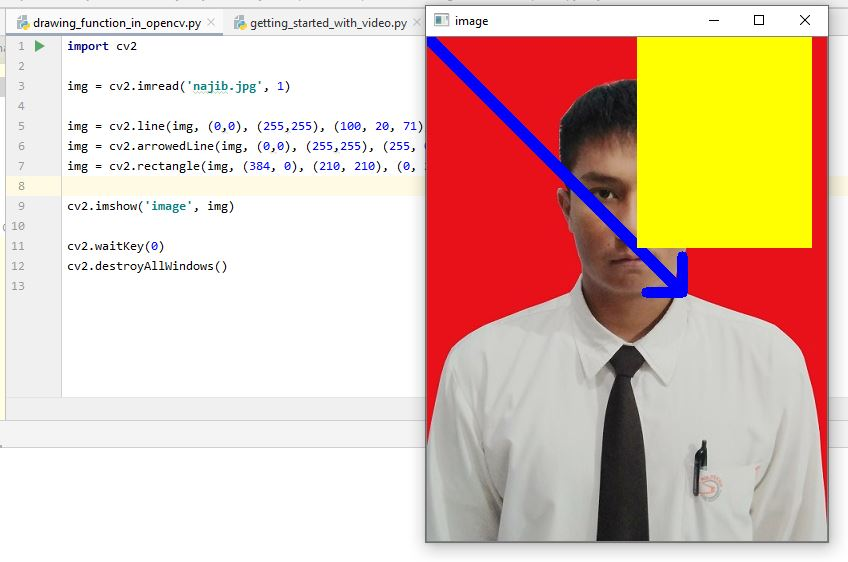
\includegraphics[scale=0.5]{figures/2,12.jpg}
\caption{Membuat kotak}
\label{contoh}
\end{figure}

Garis kotak ini bisa kita atur mau warna yang bagaimana, ukuran yang bagaimana, dan posisi yang bagaimana sesuai yang di inginkan dan sesuai kebutuhannya.

\newpage
\subsection{Membuat garis Lingkaran}
\lstinputlisting{src/cv13.py}
\begin{enumerate}
	\item lakukan Import library open cv yaitu cv2
	\item kemudian panggil file foto menggunakan kode seperti di atas, membuat terlebihdahulu variabel img, kemudian cv2.imread nama file dan nomor untuk gradiasi warnanya, pada bagian ini menggunakan angka 1 yang artinya mengikuti foto aslinya.
	\item kemudian buat garis menggunakan cv2.line, 0,0 merupakan dimana titik awal garis tersebut dan 255,255 merupakan titik akhir dari garis tersebut, kemudian selanjutnya adalah warna dari garis tersebut, dan yang terakhir adalah ketebalan dari garis yang dibuat.
	\item kemudian buat garis panah menggunakan cv2.arrowedLine, 0,0 merupakan dimana titik awal garis tersebut dan 255,255 merupakan titik akhir dari garis tersebut, kemudian selanjutnya adalah warna dari garis tersebut, dan yang terakhir adalah ketebalan dari garis yang dibuat.
	\item kemudian buat garis kotak menggunakan cv2.rectangle, 384,0 merupakan dimana titik awal garis tersebut dan 210,210 merupakan titik akhir dari garis tersebut, kemudian selanjutnya adalah warna dari garis tersebut, dan yang terakhir adalah ketebalan dari garis yang dibuat.
	\item kemudian buat garis kotak menggunakan cv2.circle, 320,63 merupakan dimana titik awal garis tersebut dan 63 merupakan titik tengah, kemudian selanjutnya adalah warna dari garis tersebut, dan yang terakhir adalah -1 yang membuat kotak terisi full karna jika plus yang membesar adalah bagian luarnya juka min yang membesar adalah bagian dalamnya jika minus maka akan full.
	\item kemudian buat frame untuk menampilkan gambar menggunakan imshow dengan nama frame image.
	\item kemudian gunakan waitKey untuk membuat frame agar tidak langsung mati atau tertutup otomatis.
	\item destroyAllWindows digunakan untuk menutup frame.
\end{enumerate}

\begin{figure}[ht]
\centering
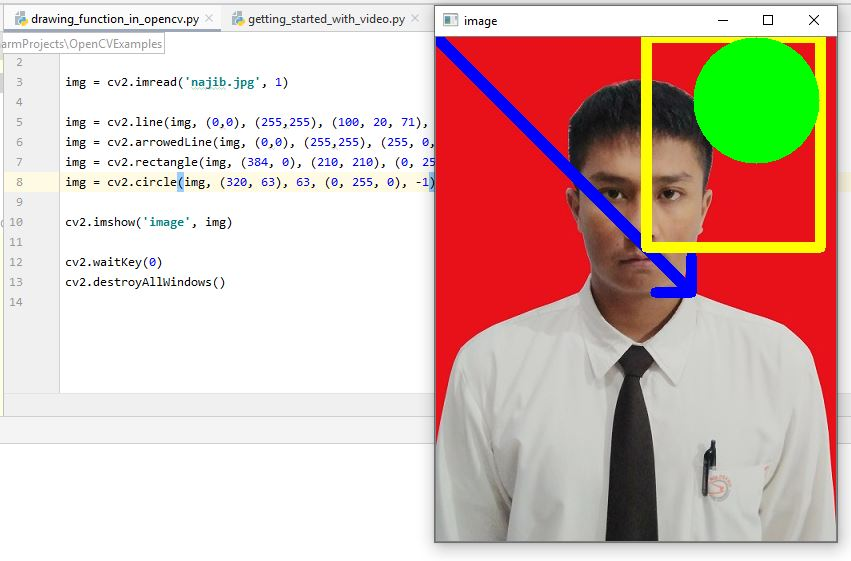
\includegraphics[scale=0.5]{figures/2,13.jpg}
\caption{Membuat garis lingkaran}
\label{contoh}
\end{figure}

Garis Lingkaran ini bisa kita atur mau warna yang bagaimana, ukuran yang bagaimana, dan posisi yang bagaimana sesuai yang di inginkan dan sesuai kebutuhannya.

\newpage
\subsection{Membuat Text}
\lstinputlisting{src/cv14.py}
\begin{enumerate}
	\item lakukan Import library open cv yaitu cv2
	\item kemudian panggil file foto menggunakan kode seperti di atas, membuat terlebihdahulu variabel img, kemudian cv2.imread nama file dan nomor untuk gradiasi warnanya, pada bagian ini menggunakan angka 1 yang artinya mengikuti foto aslinya.
	\item kemudian buat garis menggunakan cv2.line, 0,0 merupakan dimana titik awal garis tersebut dan 255,255 merupakan titik akhir dari garis tersebut, kemudian selanjutnya adalah warna dari garis tersebut, dan yang terakhir adalah ketebalan dari garis yang dibuat.
	\item kemudian buat garis panah menggunakan cv2.arrowedLine, 0,0 merupakan dimana titik awal garis tersebut dan 255,255 merupakan titik akhir dari garis tersebut, kemudian selanjutnya adalah warna dari garis tersebut, dan yang terakhir adalah ketebalan dari garis yang dibuat.
	\item kemudian buat garis kotak menggunakan cv2.rectangle, 384,0 merupakan dimana titik awal garis tersebut dan 210,210 merupakan titik akhir dari garis tersebut, kemudian selanjutnya adalah warna dari garis tersebut, dan yang terakhir adalah ketebalan dari garis yang dibuat.
	\item kemudian buat garis kotak menggunakan cv2.circle, 320,63 merupakan dimana titik awal garis tersebut dan 63 merupakan titik tengah, kemudian selanjutnya adalah warna dari garis tersebut, dan yang terakhir adalah -1 yang membuat kotak terisi full karna jika plus yang membesar adalah bagian luarnya juka min yang membesar adalah bagian dalamnya jika minus maka akan full.
	\item tentukan fontnya terlebih dahulu
	\item kemudian gunakan putText atur sesuai seperti pada gambar.
	\item kemudian buat frame untuk menampilkan gambar menggunakan imshow dengan nama frame image.
	\item kemudian gunakan waitKey untuk membuat frame agar tidak langsung mati atau tertutup otomatis.
	\item destroyAllWindows digunakan untuk menutup frame.
\end{enumerate}

\begin{figure}[ht]
\centering
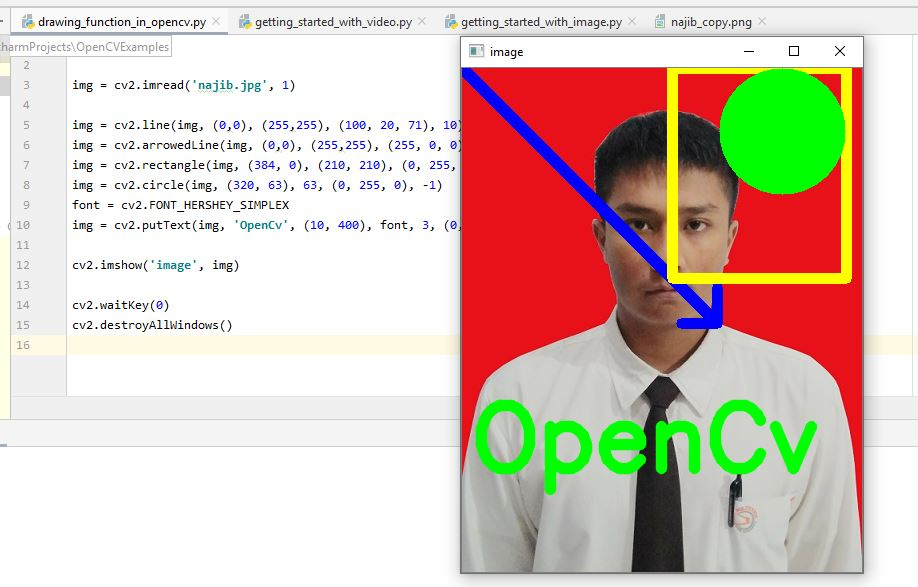
\includegraphics[scale=0.5]{figures/2,14.jpg}
\caption{Membuat Text}
\label{contoh}
\end{figure}

Text ini bisa kita buat sesuai kata kata yang di inginkan dan kata kata yang sesuai pada gambar, mau warna yang bagaimana, ukuran yang bagaimana, dan posisi yang bagaimana sesuai yang di inginkan dan sesuai kebutuhannya.

\newpage
\section{Frame Numpay}
\subsection{Membuat Frame menggunakan Numpay}
\lstinputlisting{src/cv15.py}
\begin{enumerate}
	\item lakukan import numpay as np
	\item lakukan Import library open cv yaitu cv2
	\item kemudian buat frame dari numpy yaitu zeros, kemudian ukuran fram dan warna dari fram, yang di buat adalah hitam.
	\item kemudian buat garis menggunakan cv2.line, 0,0 merupakan dimana titik awal garis tersebut dan 255,255 merupakan titik akhir dari garis tersebut, kemudian selanjutnya adalah warna dari garis tersebut, dan yang terakhir adalah ketebalan dari garis yang dibuat.
	\item kemudian buat garis panah menggunakan cv2.arrowedLine, 0,0 merupakan dimana titik awal garis tersebut dan 255,255 merupakan titik akhir dari garis tersebut, kemudian selanjutnya adalah warna dari garis tersebut, dan yang terakhir adalah ketebalan dari garis yang dibuat.
	\item kemudian buat garis kotak menggunakan cv2.rectangle, 384,0 merupakan dimana titik awal garis tersebut dan 210,210 merupakan titik akhir dari garis tersebut, kemudian selanjutnya adalah warna dari garis tersebut, dan yang terakhir adalah ketebalan dari garis yang dibuat.
	\item kemudian buat garis kotak menggunakan cv2.circle, 320,63 merupakan dimana titik awal garis tersebut dan 63 merupakan titik tengah, kemudian selanjutnya adalah warna dari garis tersebut, dan yang terakhir adalah -1 yang membuat kotak terisi full karna jika plus yang membesar adalah bagian luarnya juka min yang membesar adalah bagian dalamnya jika minus maka akan full.
	\item tentukan fontnya terlebih dahulu
	\item kemudian gunakan putText atur sesuai seperti pada gambar.
	\item kemudian buat frame untuk menampilkan gambar menggunakan imshow dengan nama frame image.
	\item kemudian gunakan waitKey untuk membuat frame agar tidak langsung mati atau tertutup otomatis.
	\item destroyAllWindows digunakan untuk menutup frame.
\end{enumerate}

\begin{figure}[ht]
\centering
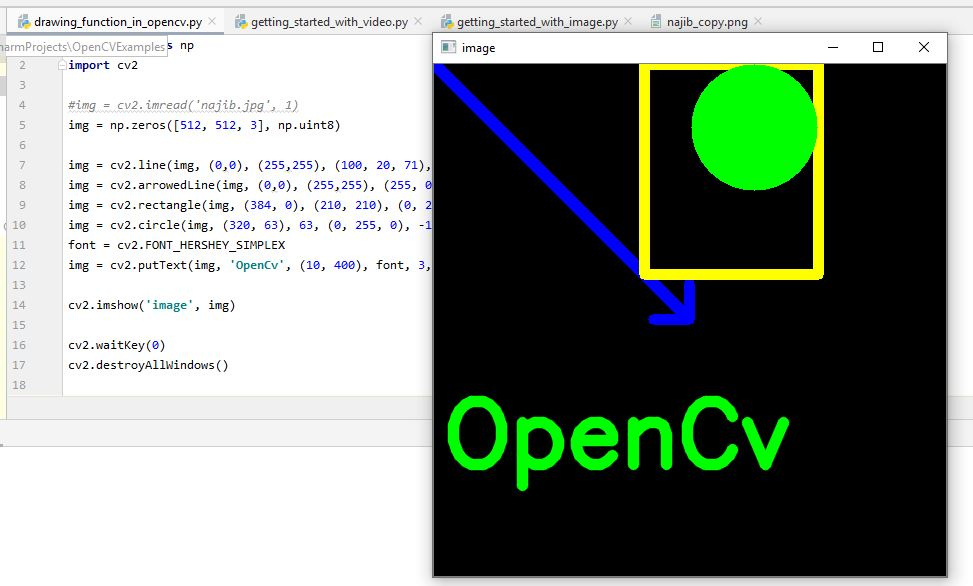
\includegraphics[scale=0.5]{figures/2,15.jpg}
\caption{Membuat Frame Numpy}
\label{contoh}
\end{figure}

Frame ini dibuat menggunakan matriks yang ada pada library numpay, kita tidak perlu lagi menghitung berapa matriksnya kita cukup gunakan zeros dan ukuran yang di butuhkan.